\noindent
En la figura~\ref{fig:diagrama-articulos-ano-metrica} se pueden visualizar las métricas de calidad, separadas por los últimos 3 años y mostrando el promedio en cada métrica de los artículos publicados en esos años, así como un apartado donde se calcula la sumatoria de estas métricas por cada año.
\begin{figure}[H]
    \centering
    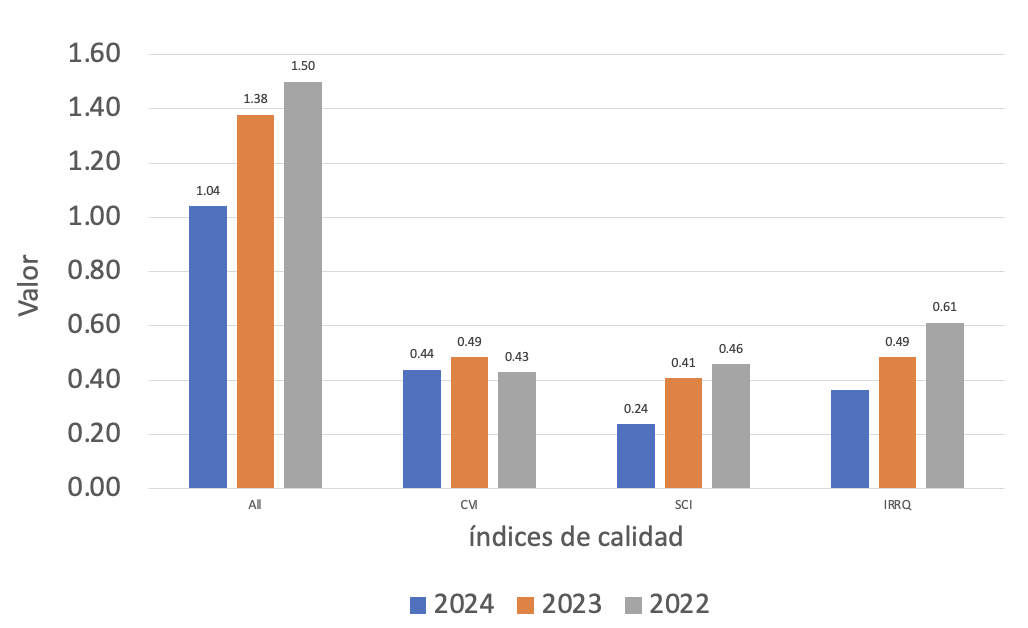
\includegraphics[scale=0.7]{tablas-images/cp2/diagrama-articulos-ano-metrica.png}
    \caption{Artículos por métricas y año}\label{fig:diagrama-articulos-ano-metrica}
\end{figure}
\noindent
En la figura~\ref{fig:tipos-articulos} se muestra el conteo de artículos por su tipo específico, el cual puede ser uno de 3 opciones: ``Revista'', ``Conferencia'' o ``Genérico''. Vemos que la mayoría de artículos provienen de revistas.
\begin{figure}[H]
    \centering
    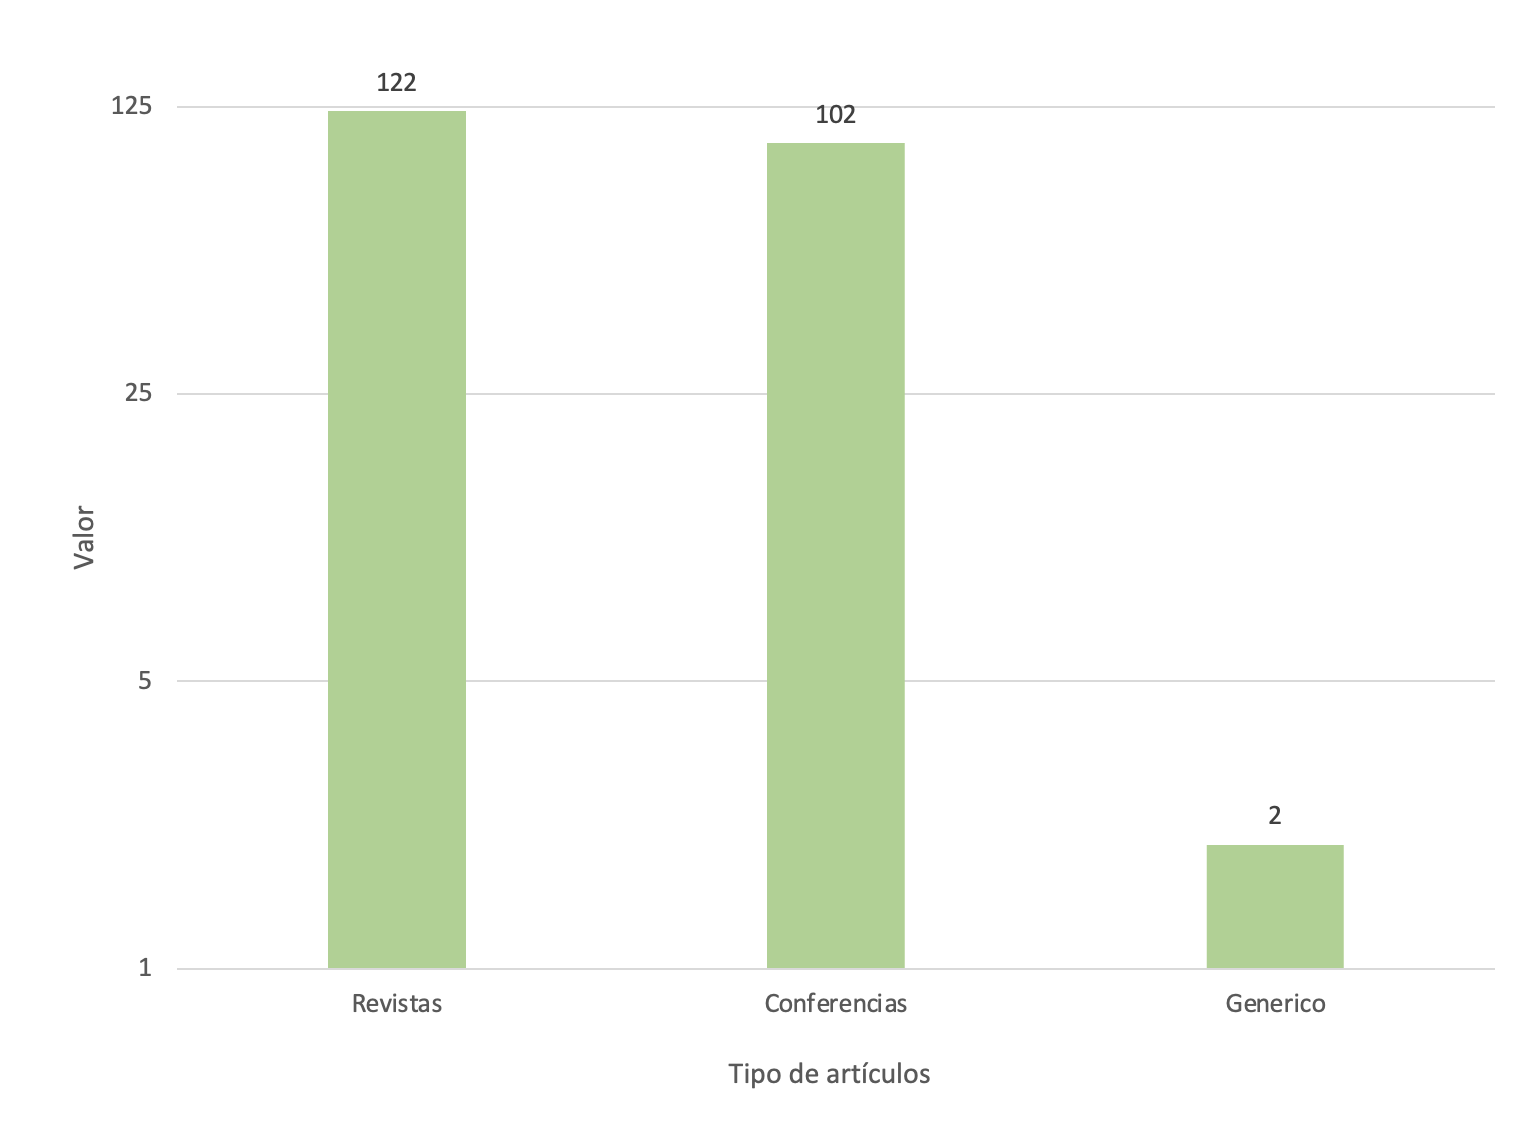
\includegraphics[scale=0.4]{tablas-images/cp2/tipos-articulos.png}
    \caption{Artículos por tipo}\label{fig:tipos-articulos}
\end{figure}
\noindent
En la figura~\ref{fig:estrategia-busqueda-articulos} se detalla la cantidad de artículos que se extrajeron de cada estrategia. Se puede observar que la estrategia que generó más artículos fue la técnica de~\textit{Snowball}. Además, es importante destacar que la inclusión directa se está contabilizando como una estrategia, ya que se consideraron artículos que no fueron encontrados en las bases de datos, pero que se conocían de antemano y cumplían con los criterios de inclusión, debido a que no fue hallado ni en las bases de datos ni en la técnica de~\textit{Snowball}.
\begin{figure}[H]
    \centering
    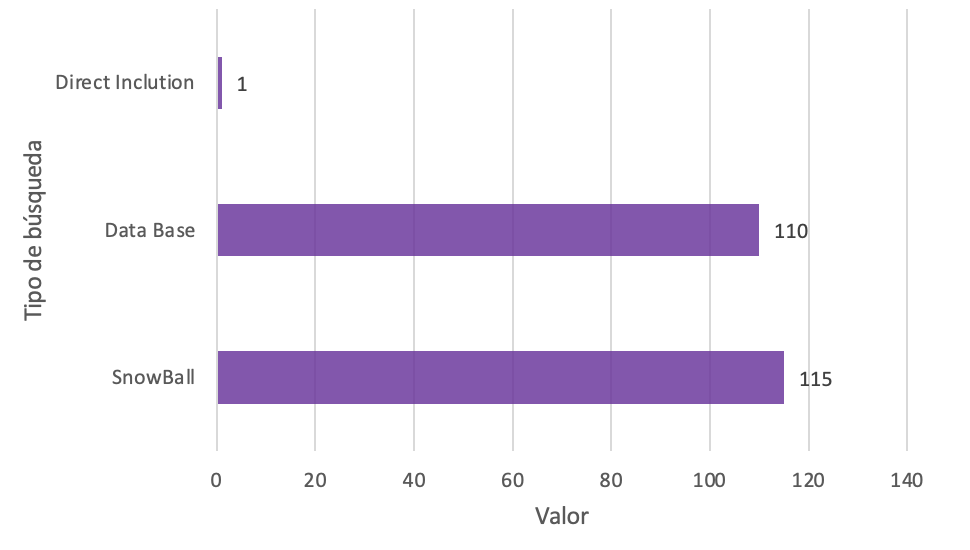
\includegraphics[scale=0.8]{tablas-images/cp2/estrategia-busqueda-articulos.png}
    \caption{Estrategia de búsqueda de artículos}\label{fig:estrategia-busqueda-articulos}
\end{figure}
\noindent
Finalmente, en la figura~\ref{fig:diagrama-red-articulos} se puede apreciar un diagrama de red, que segrega por colores los tópicos más relacionados entre sí, vemos 4 grandes grupos: IA, cloud computing, virtualización, desarrollo de software. Además permite observar qué tópicos están más relacionados entre sí, por ejemplo, se puede ver que los microservicios están muy relacionados con la computación en la nube y con Docker. La herramienta utilizada para generar este diagrama fue \textit{VOSviewer}~\citep{vosviewer_website} que permite crear mapas basados en la co-ocurrencia de términos en los artículos, y que es comúnmente utilizada para análisis bibliométricos. Basta con importar los artículos en formato \textit{RIS} o \textit{BibTeX} y la herramienta genera el diagrama automáticamente.
\begin{figure}[H]
    \centering
    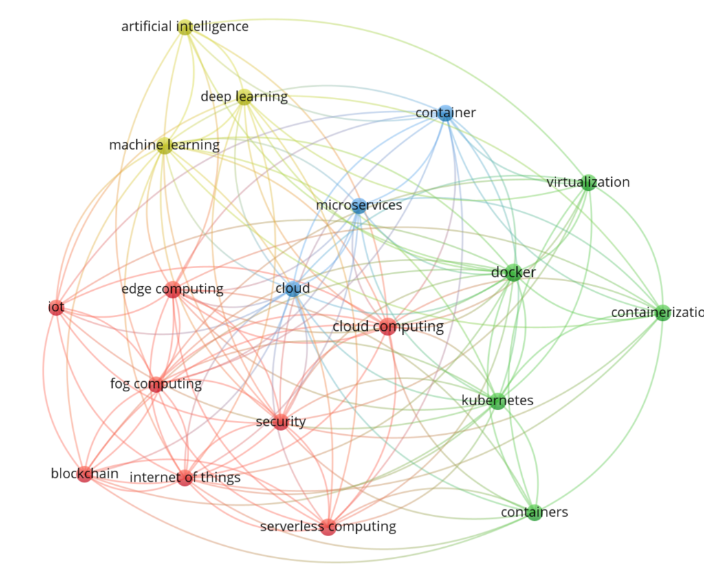
\includegraphics[scale=0.8]{tablas-images/cp2/diagrama-red-busqueda.png}
    \caption{Diagrama de red de los artículos}\label{fig:diagrama-red-articulos}
\end{figure}